\section{Konfiguracja}
\label{sec:konfiguracja}

\par Zaimplementowane rozwiązanie posiada wiele elementów wymagających skonfigurowania. Od podstawowej konfiguracji działających w nim mikroserwisów, poprzez konfigurację infrastruktury, aż do dostarczenia odpowiednich plików map.

\subsection{Warstwy konfiguracji i ustawiania współdzielone}

\par Ze względu na współdzielenie dużej części kodu pomiędzy wieloma mikroserwisami, również część ich konfiguracji musiała być współdzielona\english{Shared}. Współdzielenie to odbywa się przy wykorzystaniu plików \texttt{sharedsettings.*.json}. Pliki te zawierają ustawienia wykorzystywane przez wszystkie mikroserwisy w systemie. Przykładem takich ustawień może być konfiguracja związana z infrastrukturą. Tabela \ref{tab:configurationSharedSettings} przedstawia wykaz ustawień współdzielonych, wraz z ich znaczeniem.

\begin{table}[H]
    \centering
    \begin{tabular}{|p{0.5\linewidth} | p{0.5\linewidth}|} 
     \hline
     Ustawienie & Znaczenie \\
     \hline
     \hline
     RabbitMq.Host & Host \emph{RabbitMQ} \\ 
     \hline
     RabbitMq.Port & Port \emph{RabbitMQ} \\ 
     \hline
     RabbitMq.Username & Nazwa użytkownika \emph{RabbitMQ} \\ 
     \hline
     RabbitMq.Password & Hasło \emph{RabbitMQ} \\ 
     \hline
     RabbitMq.MessageExchange & Nazwa giełdy dla wiadomości wysyłanych między agentami \\ 
     \hline
     RabbitMq.DirectMessageExchange & Nazwa giełdy dla bezpośrednich wiadomości wysyłanych między agentami \\ 
     \hline
     RabbitMq.EventExchange & Nazwa giełdy dla wydarzeń \\ 
     \hline
     RabbitMq.QueryExchange & Nazwa giełdy dla kwerend \\ 
     \hline
     RabbitMq.CommandExchange & Nazwa giełdy dla komend \\ 
     \hline
     Loki.Uri & URI \emph{Loki}ego \\ 
     \hline
     Loki.Login & Nazwa użytkownika \emph{Loki}ego \\ 
     \hline
     Loki.Password & Hasło \emph{Loki}ego \\ 
     \hline
     SimulationCommunicationSettings.Host & Host \emph{RabbitMQ} dla komunikacji z symulacją \\ 
     \hline
     SimulationCommunicationSettings.Port & Hasło \emph{RabbitMQ} dla komunikacji z symulacją \\ 
     \hline
     SimulationCommunicationSettings.Username & Nazwa użytkownika \emph{RabbitMQ} dla komunikacji z symulacją \\ 
     \hline
     SimulationCommunicationSettings.Password & Hasło \emph{RabbitMQ} dla komunikacji z symulacją \\ 
     \hline
     ServiceSettings.Id & Identyfikator serwisu typu \texttt{GUID} \\ 
     \hline
     ServiceSettings.ServiceType & Typ serwisu. Możliwe wartości: \texttt{HqService}, \texttt{PatrolService}, \texttt{GunService}, \texttt{NavigationService} i \texttt{WebApi}. \\ 
     \hline
    \end{tabular}
    \caption{Wykaz ustawień współdzielonych}
    \label{tab:configurationSharedSettings}
\end{table}

\par Wszystkie te ustawienia mogą jednak zostać nadpisane. Zastosowany został tutaj model warstwowy, gdzie ustawienia z wyższych warstw nadpisują te z niższych. Model warstw przedstawia diagram \ref{fig:configurationLayersModel}. Zaznaczone w nim \texttt{ENVIRONMENT} oznacza zmienną określającą środowisko w jakim aplikacja została uruchomiona. Można ją ustawić za pomocą argumentu \texttt{--environment=ENVIRONMENT} podczas uruchamiania \texttt{dotnet} lub poprzez ustawienie zmiennej środowiskowej \texttt{ASPNETCORE\_ENVIRONMENT} w swoim systemie\cite{MSDOCS_DOTNET_ENVIRONMENTS}.

\par Przykładem zastosowania mechanizmu nadpisywania zmiennych mogą być \texttt{ServiceSettings}. Korzysta z nich każdy serwis działający w aplikacji, jednak są to ustawienia identyfikujące - dlatego znajdują się w \texttt{appsettings.json} konkretnych serwisów.

\par Każde pole konfiguracji może również zostać nadpisane wykorzystując zmienne środowiskowe. Aby uniknąć potencjalnych konfliktów z możliwymi istniejącymi już nazwami, postanowiono dodać \emph{prefix} \texttt{PoliceSupportSystem\_}. Przykładowa nazwa zmiennej środowiskowej powinna wyglądać w następujący sposób: \texttt{PoliceSupportSystem\_ServiceSettings\_\_Id}.

\begin{figure}
    \centering
    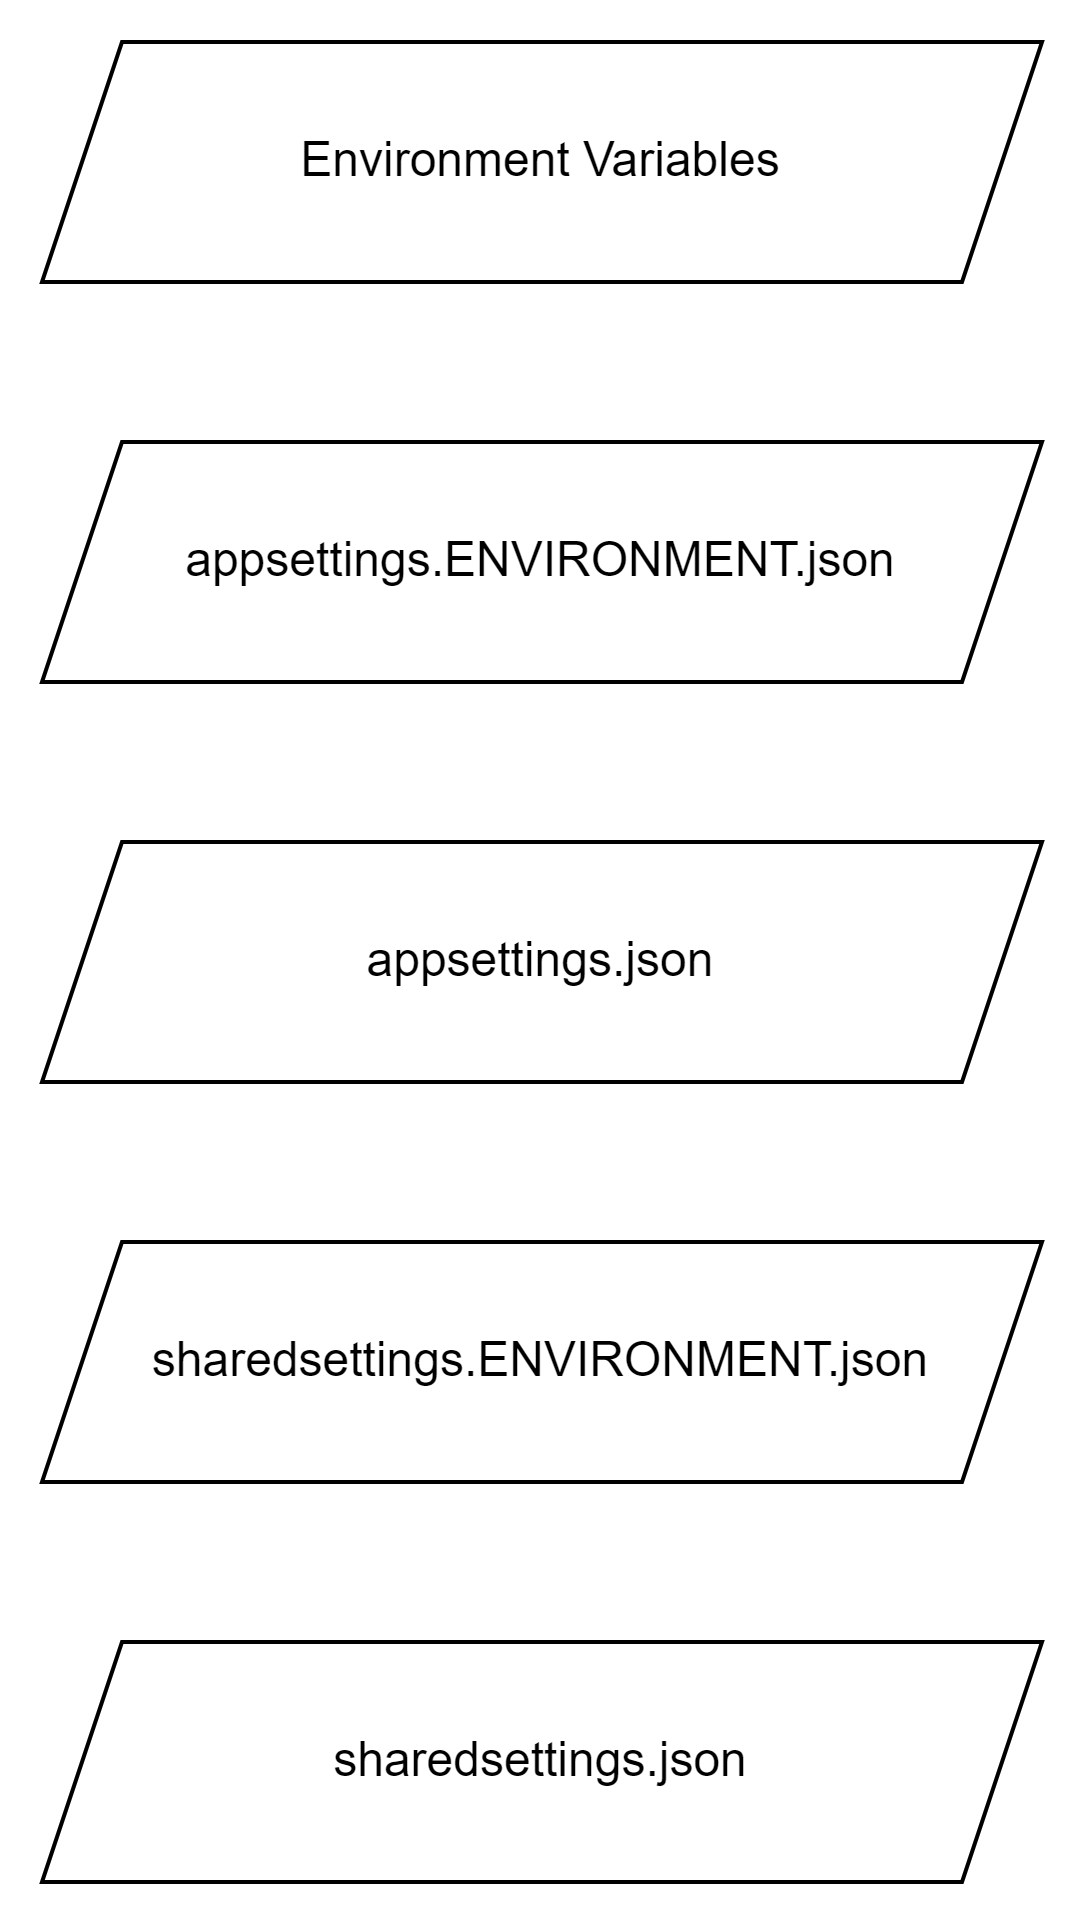
\includegraphics[height=\linewidth]{Configuration - Layers Model}
    \caption{Warstwy konfiguracji}
    \label{fig:configurationLayersModel}
    \source{Opracowanie Własne}
\end{figure}

\subsection{Konfiguracja serwisów i działających w nich agentów}

\par Jedyne ustawienia wymagane do konfiguracji w \emph{Web App} to \texttt{MapSettings}. Zostały one opisane w tabeli \ref{tab:configurationWebAppSettings}.

\begin{table}[H]
    \centering
    \begin{tabular}{|p{0.5\linewidth} | p{0.5\linewidth}|} 
     \hline
     Ustawienie & Znaczenie \\
     \hline
     \hline
     MapSettings.HqLocation.Latitude & Szerokość geograficzna lokalizacji kwatery głównej. Typ: \texttt{double}. \\ 
     \hline
     MapSettings.HqLocation.Longitude & Długość geograficzna lokalizacji kwatery głównej. Typ: \texttt{double}. \\ 
     \hline
    \end{tabular}
    \caption{Ustawienie specyficzne dla \emph{Web App}}
    \label{tab:configurationWebAppSettings}
\end{table}

\par \emph{HQ Service} wymaga skonfigurowania \texttt{HqAgentSettings} i \texttt{DecisionServiceSettings}. Możliwe ustawienia przedstawia tabela \ref{tab:configurationHqServiceSettings}.

\begin{table}[H]
    \centering
    \begin{tabular}{|p{0.5\linewidth} | p{0.5\linewidth}|} 
     \hline
     Ustawienie & Znaczenie \\
     \hline
     \hline
     HqAgentSettings.HqAgentId & Identyfikator \emph{HQ Agent}. Typ: \texttt{GUID}. \\ 
     \hline
     DecisionServiceSettings.EvenPatrolDistribution & Kontroluje przydział patroli do dzielnic. Równomierne lub zależne od \emph{DistrictDangerLevels}. Typ: \texttt{bool}. \\ 
     \hline
     DecisionServiceSettings.DistanceWeight & Waga dla cechy: dystans w algorytmie decyzyjnym. Typ: \texttt{double}. \\ 
     \hline
     DecisionServiceSettings.SameDistrictWeight & Waga dla cechy: patrol w tej samej dzielnicy. Typ: \texttt{double}. \\ 
     \hline
     \makecell[tl]{DecisionServiceSettings\\.InsufficientNumberOfPatrolsInDistrictWeight} & Waga dla cechy: przydział patrolu oddali od wymaganej ilości patroli w dzielnicy, o określonym poziomie niebezpieczeństwa. Typ: \texttt{double}. \\ 
     \hline
     DecisionServiceSettings.DistrictDangerLevels & Słownik zawierający poziomy niebezpieczeństwa dla dzielnic. Typ: \texttt{Dictionary<string, DistrictDangerLevelEnum>}. \\ 
     \hline
     \makecell[tl]{DecisionServiceSettings\\.DangerLevelRequiredPatrollingPatrols} & Ilość wymaganych patroli w zależności od poziomu niebezpieczeństwa dzielnicy. Wpływa na cechę, kontrolowaną przez \texttt{InsufficientNumberOf PatrolsInDistrictWeight}. Typ:\newline \texttt{Dictionary <DistrictDangerLevelEnum,int>}. \\ 
     \hline
    \end{tabular}
    \caption{Ustawienie specyficzne dla \emph{HQ Service}}
    \label{tab:configurationHqServiceSettings}
\end{table}

\par \emph{Patrol Service}, \emph{Navigation Service} i \emph{Gun Service} wymagają skonfigurowania \texttt{PatrolSettings}. Dostępne ustawiania przedstawia tabela \ref{tab:configurationPatrolServiceSettings}.

\begin{table}[H]
    \centering
    \begin{tabular}{|p{0.5\linewidth} | p{0.5\linewidth}|} 
     \hline
     Ustawienie & Znaczenie \\
     \hline
     \hline
     PatrolSettings.PatrolId & Identyfikator patrolu. Typ: \texttt{int}. \\ 
     \hline
     PatrolSettings.PatrolAgentId & Identyfikator \emph{Patrol Agent}. Typ: \texttt{GUID}. \\ 
     \hline
     PatrolSettings.NavigationAgentId & Identyfikator \emph{Navigation Agent}. Typ: \texttt{GUID}. \\ 
     \hline
     PatrolSettings.GunAgentId & Identyfikator \emph{Gun Agent}. Typ: \texttt{GUID}. \\ 
     \hline
    \end{tabular}
    \caption{Ustawienie specyficzne dla patroli}
    \label{tab:configurationPatrolServiceSettings}
\end{table}


\subsection{Konfiguracja symulacji}

\par Jako iż symulacja jest osobną aplikacją i nie posiada żadnych części współdzielonych z pozostałymi serwisami (poza biblioteką \texttt{Simulation.Communication} definiującą wiadomości, które symulacja wysyła i odbiera), to nie wpływają na nią ustawienia z \texttt{sharedsettings.json}. Jedynym źródłem jej konfiguracji, są powiązane z nią pliki \texttt{appsettings.*.json}. Pełen wykaz możliwych ustawień prezentuje tabela \ref{tab:configurationSimulationSettings}.


\begin{longtable}{|p{0.5\linewidth} | p{0.5\linewidth}|} 
     \hline
     Ustawienie & Znaczenie \\
     \hline
     \hline
     SimulationSettings.TimeRate & Definiuje o ile razy szybciej powinien płynąć czas w symulacji, niż w rzeczywistości. Typ: \texttt{double}. \\ 
     \hline
     SimulationSettings.StartDelay & Opóźnienie startu symulacji. Typ: \texttt{TimeSpan?}. \\ 
     \hline
     SimulationSettings.EndAfterSimulationTime & Czas w symulacji, po jakim powinno nastąpić jej zatrzymanie. Typ: \texttt{TimeSpan?}. \\ 
     \hline
     SimulationSettings.HqLocation.Latitude & Szerokość geograficzna lokalizacji kwatery głównej. Typ: \texttt{double}. \\ 
     \hline
     SimulationSettings.HqLocation.Longitude & Długość geograficzna lokalizacji kwatery głównej. Typ: \texttt{double}. \\ 
     \hline
     IncidentDirectorSettings.DistrictDangerLevels & Słownik zawierający konfigurację poziomu niebezpieczeństwa danej dzielnicy. Typ: \texttt{Dictionary<string, DistrictDangerLevelEnum>}, gdzie \texttt{DistrictDangerLevelEnum} może posiadać wartości: \texttt{Low}, \texttt{Normal} i \texttt{High}. \\ 
     \hline
     \makecell[tl]{IncidentDirectorSettings\\.DangerLevelShootingChance.Low} & Szansa na przerodzenie się incydentu w strzelaninę w dzielnicy z \texttt{DistrictDangerLevel} równym \texttt{Low}. Typ: \texttt{double}, wartości $[0, 1]$. \\ 
     \hline
     \makecell[tl]{IncidentDirectorSettings\\.DangerLevelShootingChance.Normal} & Szansa na przerodzenie się incydentu w strzelaninę w dzielnicy z \texttt{DistrictDangerLevel} równym \texttt{Normal}. Typ: \texttt{double}, wartości $[0, 1]$. \\ 
     \hline
     \makecell[tl]{IncidentDirectorSettings\\.DangerLevelShootingChance.High} & Szansa na przerodzenie się incydentu w strzelaninę w dzielnicy z \texttt{DistrictDangerLevel} równym \texttt{High}. Typ: \texttt{double}, wartości $[0, 1]$. \\ 
     \hline
     \makecell[tl]{IncidentDirectorSettings\\.DangerLevelMaxNumberOfIncidentPerDay\\.Low} & Maksymalna ilość incydentów w ciągu dnia dla dzielnicy z \texttt{DistrictDangerLevel} równym \texttt{Low}. Typ: \texttt{int}. \\ 
     \hline
     \makecell[tl]{IncidentDirectorSettings\\.DangerLevelMaxNumberOfIncidentPerDay\\.Normal} & Maksymalna ilość incydentów w ciągu dnia dla dzielnicy z \texttt{DistrictDangerLevel} równym \texttt{Normal}. Typ: \texttt{int}. \\ 
     \hline
     \makecell[tl]{IncidentDirectorSettings\\.DangerLevelMaxNumberOfIncidentPerDay\\.High} & Maksymalna ilość incydentów w ciągu dnia dla dzielnicy z \texttt{DistrictDangerLevel} równym \texttt{High}. Typ: \texttt{int}. \\ 
     \hline
     PatrolDirectorSettings.NormalPatrolSpeed & Prędkość patrolu wyrażona w $km/h$ w warunkach normalnych. Typ: \texttt{double}. \\ 
     \hline
     PatrolDirectorSettings.EmergencyPatrolSpeed & Prędkość patrolu wyrażona w $km/h$ w warunkach specjalnych. Typ: \texttt{double}. \\ 
     \hline 
     RabbitMqSettings.Host & Host \emph{RabbitMQ} \\ 
     \hline 
     RabbitMqSettings.Port & Port \emph{RabbitMQ} \\ 
     \hline 
     RabbitMqSettings.Username & Nazwa użytkownika \emph{RabbitMQ} \\ 
     \hline 
     RabbitMqSettings.Password & Hasło \emph{RabbitMQ} \\ 
     \hline 
     LokiSettings.Uri & URI \emph{Loki}ego \\ 
     \hline 
     LokiSettings.Login & Nazwa użytkownika \emph{Loki}ego \\ 
     \hline
     LokiSettings.Password & Hasło \emph{Loki}ego \\ 
     \hline
     DbSettings.Host & Host \emph{PostgreSQL} \\ 
     \hline
     DbSettings.Port & Port \emph{PostgreSQL} \\ 
     \hline
     DbSettings.Username & Nazwa użytkownika \emph{PostgreSQL} \\ 
     \hline
     DbSettings.Password & Hasło \emph{PostgreSQL} \\ 
     \hline
     DbSettings.DbName & Nazwa bazy danych \emph{PostgreSQL} zawierającej zaimportowane dane. \\ 
     \hline
\caption{Wykaz ustawień symulacji}
\label{tab:configurationSimulationSettings}
\end{longtable}


\subsection{Docker}

\par Konfiguracja niektórych serwisów odbywa się w plikach \emph{Docker Compose}\cite{DOCKER_COMPOSE_DOCS}. W tym celu korzysta się z możliwości ustawienia zmiennych środowiskowych dla danego kontenera. Jest to sekcja \texttt{environment} danego pliku \emph{compose}.

\par Import map odbywa się na bazie konfiguracji w pliku \texttt{infrastructure-docker-compose.yaml}. Aby poprawnie zaimportować przygotowane pliki map, musimy w je wskazać w zmiennych środowiskowych \texttt{MAP\_FILE} i \texttt{DISTRICTS\_FILE} oraz umieścić w folderze \texttt{./SimulationDb/maps}.

\par Mechanizm ten jest również wykorzystywany przy konfiguracji patroli, biorących udział w działaniu systemu. Aby dodać patrol należy go zdefiniować w pliku \texttt{docker-compose.yaml}. Konfiguracja ta wykorzystuje zmienne środowiskowe, aby ustawić odpowiednie identyfikatory serwisom patrolu. Zostało to dokładniej opisane w podrozdziale \ref{sec:konteneryzacjaSystemu}.

